\documentclass[12pt,a4paper]{scrartcl}

\usepackage[utf8]{inputenc}
\usepackage{german}
%\usepackage[latin1]{inputenc}
\usepackage{graphicx}
\usepackage{amsfonts}
\usepackage{amsmath}
\usepackage{amssymb}
\usepackage{color}
\usepackage{hyperref}
\usepackage{alltt}
\usepackage{enumerate}
\usepackage{hyperref}

\usepackage{listings}
\lstdefinelanguage{Racket}
{
	keywords=
	{
		define, lambda, cond, if, else, send
	} ,
	comment=[l]{;}
}
\lstset
{
	language=Racket,
	keywordstyle=\bfseries ,
	commentstyle=\color{blue}\itshape,
	basicstyle =\rmfamily\color{black}\small
}

\setlength{\parindent}{0pt}

\sloppy
\parindent0cm
\parskip0.2cm

\newcommand\HR{\rule{175mm}{0.4pt}}

\hypersetup
{
	pdfauthor={Christian Wagenknecht},
	pdftitle={\"{U}bung},
	pdfsubject={Rekursive Prozeduren, Teil 1},
	pdfkeywords={Racket}
}

\hypersetup
{
	pdfpagemode=Fullscreen,
	colorlinks=true
}

\definecolor{brown}{rgb}{0.8,0.4,0.1}

%-------------------------------------------------------------------------------

\begin{document}
\begin{minipage}[b]{174mm}
  \begin{minipage}[t]{80mm}
    \par\vspace{0mm}
    \textcolor{blue}{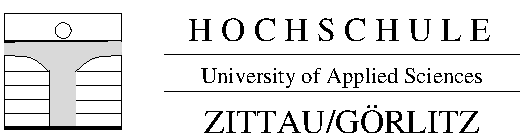
\includegraphics[scale=0.8]{fh-logo.pdf}}
  \end{minipage}\hfill
  \begin{minipage}[t]{76mm}                      % 120mm
    \par\vspace{2mm}
    {\sc Fachbereich Informatik}\\
    {\sc Prof.~Dr.~Christian~Wagenknecht}\\
    \par
    \textbf{Programmierparadigmen, \"{U}bung 3}
  \end{minipage}
\end{minipage}
\HR

%-------------------------------------------------------------------------------

\subsection*{\textcolor{red}{\textsc{Rekursive Prozeduren, Teil 1}}}


\subsubsection*{Verwendung des Turtle-Systems mit DrRacket}

\begin{enumerate}
\item 
Bestimmen Sie ein Arbeitsverzeichnis und kopieren Sie die Datei\\ \href{http://f-ei.hszg.de/wagenkn/PP-Racket/downloads/racket/racketturtle2014.rkt}{racketturtle2014.rkt} dort hinein.

\item 
Öffnen Sie eine neue Racket-Datei, in der Sie das Turtle-System verwenden möchten, und speichern Sie diese Datei im Arbeitsverzeichnis. F\"{u}gen Sie im Definitionsfenster die folgenden Zeilen ein:
\begin{verbatim}
#lang racket
(require "racketturtle2014.rkt")

(define width 800) ; Determines the window's size (turtles' playground)
(define height 800)

(define dc (start width height))  
\end{verbatim}
\end{enumerate}

Nun sind Sie betriebsbereit. Die Fläche, in der sich die Turtle(s) bewegen, ist mit 800 mal 800 bereits vorgegeben. 

Eine Turtle, wie etwa \texttt{harald}, wird mit folgender Anweisung (im Definitionsfenster!) instanziiert:
\begin{verbatim}
(define harald (new turtle% 
                    [tname 'Harald]
                    [xpos 400][ypos 500][direction 90]
                    [tcolor "YellowGreen"]
                    [tdc dc]))
\end{verbatim}

\texttt{harald} sitzt auf Position (400,500). Der Koordinatenursprung (0,0) befindet sich in der linken oberen Ecke. Die x-Koordinatenachse zeigt von dort nach rechts und die y-Achse zeigt nach unten. 

Noch ist Harald nicht zu sehen. Das lässt sich (durch Eingabe im Interaktionsfenster!) ändern:

\verb|> (send harald show!)|

\newpage

Das spitzwinklig-gleichschenklige Dreieck gibt die Blick- und potenzielle Bewegungsrichtung von Harald an. Wir schicken ihn z.B. 50 Schritte vorw\"{a}rts:

\verb|> (send harald forward! 50)|

Eine rote Spur seiner Bewegung wird sichtbar. An deren Ende sitzt Harald und erwartet weitere Instruktionen.

S\"{a}mtliche Kommandos, die eine Turtle (wie Harald) versteht, finden sich in der folgenden Liste. Das Aufrufmuster ist \verb|(send [turtle-name] [command])|.

\subsubsection*{Turtle-Kommandos}
\begin{tabular}{ll}
\texttt{say-your-name}  & Die Turtle nennt ihren Namen.\\
\texttt{forward! n} 	& Die Turtle läuft \texttt{n} Schritte nach vorn. \\
\texttt{backward! n} 	& Die Turtle läuft \texttt{n} Schritte zur\"{u}ck. \\
\texttt{right! a} 		& Die Turtle dreht sich um \texttt{a} Grad nach rechts. \\
\texttt{left! a} 	    & Die Turtle dreht sich um \texttt{a} Grad nach links. \\
\texttt{pen-up!} 		& Die Turtle hebt den Stift an. Die folgenden Bewegungen\\ & hinterlassen keine Spur. \\
\texttt{pen-down!} 		& Die Turtle senkt den Stift ab. Die folgenden Bewegungen\\ & hinterlassen eine Spur. \\
\texttt{pen-erase!}	    & Der Stift der Turtle verwandelt sich in einen Radierer. \\
\texttt{set-turtle-color! c}& Die Turtle \"{a}ndert die Turtle-Farbe. \\
						& M\"{o}gliche Werte: s. \href{http://docs.racket-lang.org/draw/color-database___.html?q=the-color-database}{Racket color Database} \\
\texttt{set-pen-color! c}   & Die Turtle \"{a}ndert die Stiftfarbe. \\
						& M\"{o}gliche Werte: s. \href{http://docs.racket-lang.org/draw/color-database___.html?q=the-color-database}{Racket color Database} \\
\texttt{clone} 			& Die Turtle klont sich selbst. \\
\texttt{hide!} 			& Die Turtle versteckt sich. \\
\texttt{show!} 			& Die Turtle zeigt sich wieder (an aktueller Position).\\
\texttt{crow}           & Die Turtle stößt einen Freudenschau (Glockenklang) aus.\\
\texttt{sleep n}        & Die Turtle schläft \texttt{n} Millisekunden.
\end{tabular}

Machen Sie sich mit diesen Kommandos durch aktive Kommunikation mit Harald vertraut.

\subsubsection*{Eigene Turtle-Prozeduren}

Im Folgenden werden eigene Prozeduren angegeben, die diese Grundkommandos verwenden und ganz bestimmte grafische Darstellungen erzeugen, beispielsweise ein Quadrat:

\begin{verbatim}
(define square
  (lambda (side turtle)
    (send turtle forward! side)
    (send turtle right! 90)
    (send turtle forward! side)
    (send turtle right! 90)
    (send turtle forward! side)
    (send turtle right! 90)
    (send turtle forward! side)
    (send turtle right! 90)))

> (square 100 harald)
\end{verbatim}

Im Definitionstext erkennt man die vierfache Ausführung von
\begin{verbatim}
    (send turtle forward! side)
    (send turtle right! 90)
\end{verbatim}
was zur Erzeugung eines Quadrats notwendig ist.

Um den Schreibaufwand (und damit die Fehlergefahr) zu verringern, setzen wir das Sprachelement \texttt{for} ein, das \textit{Iterationen} ermöglicht.
\begin{verbatim}
(define square2
  (lambda (side turtle)
    (for ([n (in-range 4)])
      (send turtle forward! side)
      (send turtle right! 90))))

> (square2 100 harald)
\end{verbatim}


%\lstinputlisting{rkt/square.rkt}
%\verb|> (square 100 harald)|\\
%\texttt{ready}
%
%\lstinputlisting{rkt/square2.rkt}
%\verb|> (square2 100 harald)|\\
%\texttt{ready}

\subsubsection*{Aufgaben}

\begin{enumerate}

% ---- Aufgabe 1 - rechteck ----
\item Schreiben Sie eine Prozedur, die ein Rechteck mit den Seitenl\"{a}ngen
\texttt{a} und \texttt{b} mit einer gegebenen Turtle zeichnet.

% ---- Aufgabe 2 - Haus vom Nikolaus ----
\item Schreiben Sie eine Prozedur, mit deren Hilfe das Haus vom Nikolaus gezeichnet werden kann.
Die Prozedur soll als Argumente die Turtle sowie die L\"{a}nge der Grundseite des Hauses \"{u}bernehmen.

% ---- Aufgabe 3 - kreisbogen ----
\item Schreiben Sie eine rekursive Prozedur \texttt{kreisbogen}, die eine Turtle und
die Bogenl\"{a}nge nimmt und einen dementsprechenden Kreisbogen zeichnet.

\textbf{Hinweis:} Ein Turtle-Kreis ist ein 360-Eck. Jeder der 360
Turtle-Schritte hat die L\"{a}nge 1. Nach jedem Schritt dreht sich die Turtle um 1
Grad nach rechts (oder links). Der Umfang dieses Kreises betr\"{a}gt offenbar 360.
(Ganz nebenbei: Wie gro{\ss} ist dann eigentlich der Radius?)

\newpage

% ---- Aufgabe 4 - binary tree ----
\item Erproben Sie die rekursive Prozedur \texttt{tree} aus der Vorlesung. Machen Sie sich die rekursive Idee durch Beschreibung des grafischen Resultats vollständig klar.
\begin{verbatim}
(define tree
  (lambda (side turtle)
    (if (< side 5) 
        (send turtle crow)
        (begin
          (send turtle forward! side)
          (send turtle left! 45)
          (send turtle sleep 10)
          (tree (/ side 2) turtle)
          (send turtle right! 90)
          (send turtle sleep 10)
          (tree (/ side 2) turtle)
          (send turtle left! 45)
          (send turtle backward! side)))))
         
> (tree 100 harald)    
\end{verbatim}

Vor diesem Aufruf kann man die turtle bei angehobenem Stift r\"{u}ckw\"{a}rts bewegen und dann den Stift absenken lassen.
Auf diese Weise gewinnt man auf der Zeichenfläche mehr Platz f\"{u}r die Zeichnung.
%\lstinputlisting{rkt/binary_tree.rkt}

\textbf{Hinweis:} Je nach Geschwindigkeit Ihres Rechners sollten Sie die Verz\"{o}gerung der grafischen Darstellung durch das konkrete Argument (Zahlenwert in Millisekunden) von \texttt{sleep-for-a-while} anpassen.

% ---- Aufgabe 5 - Rosetten ----
\item Lassen Sie sich von den sch\"{o}nen Rosetten (s.u.) inspirieren und entwerfen Sie \"{a}hnliche. Beginnen Sie stets mit der Planung und verbalen Beschreibung der zu zeichnenden Figuren. Die Implementierung erfolgt mit rekursiven Turtle-Prozeduren.
\begin{center}
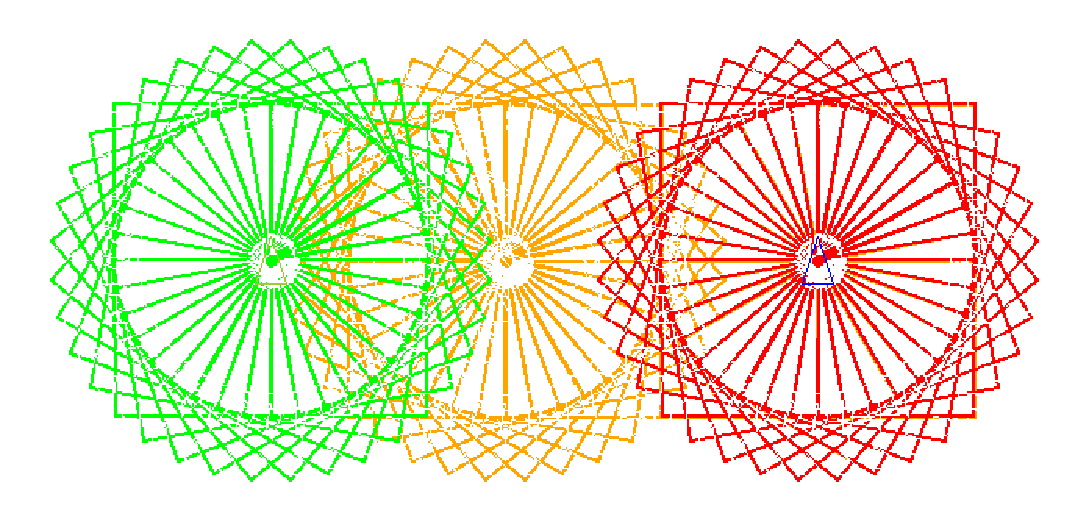
\includegraphics[width=100mm]{rosetten.pdf}
\end{center}

\end{enumerate}

\end{document} 